\chapter{Specification \& Design} \label{ch:design}

This section describes the design of the system as a website.

\section{Platform}
A web application as a platform to create visualizations takes advantage of the numerous open source visualization libraries and HTML, CSS and JavaScript are well equipped in creating interactive and visually pleasing interfaces. For these reasons, the application will take the form of a website.\par

More specifically the design will be implemented as a Django \cite{django} web application. Django is a popular Python web application. It is well documented and has numerous open source libraries which supports the creation of visualizations. Using this framework, third-party libraries could be utilized to produce JavaScript needed to create visualizations. Python\textquotesingle s machine learning libraries will be used to manipulate and analyze data.

\section{Preprocessing of data} \label{preprocessing}
Prior to the creation of the application, some preprocessing of the data must be done. The Microsoft Word document of the survey code translation in its current form is not able to be queried since it is just a Word document. It should be created as a formatted text file that is still readable for the user so that the system can query it and and in the future, the user can create the text file themselves. Inputting the translations in one file will be more user-friendly than inputting translations of individual questions through a normal form.\par

For this system design, since the user has only given the survey code translation as a Word document. I will create the formatted text file myself.\par


\begin{figure}[h]
\centering
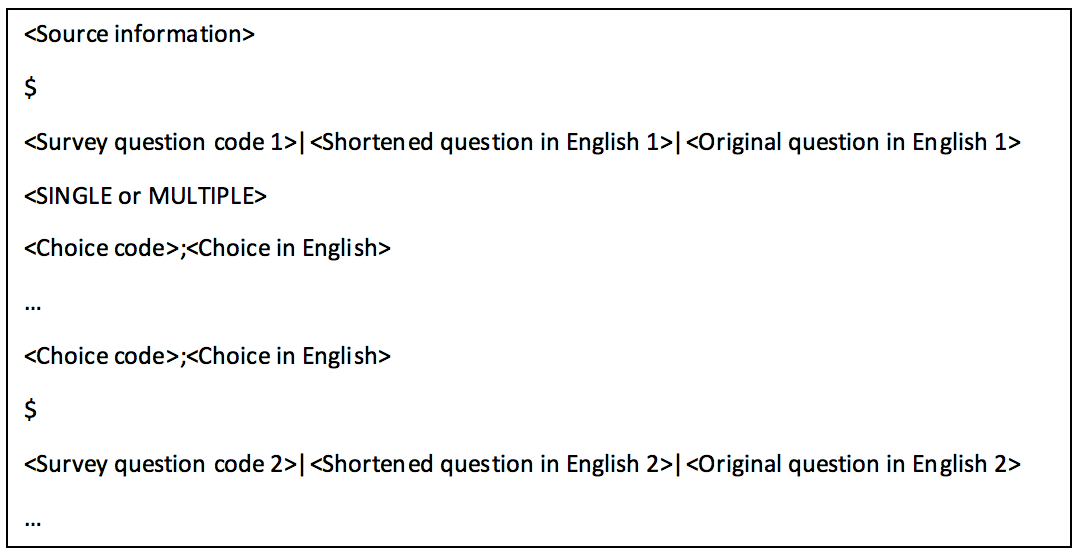
\includegraphics[scale=0.5]{textformatted}
\caption{Formatted text file of survey code translation (See Appendix for actual text)}
\end{figure}

As  seen above the text file is still readable as each question\textquotesingle s data is separated by a `\$' sign and each code is separated by a `;' or `|'. The question text is distinguishable from the choices text.

\section{System architecture}

\begin{figure}[h]
\centering
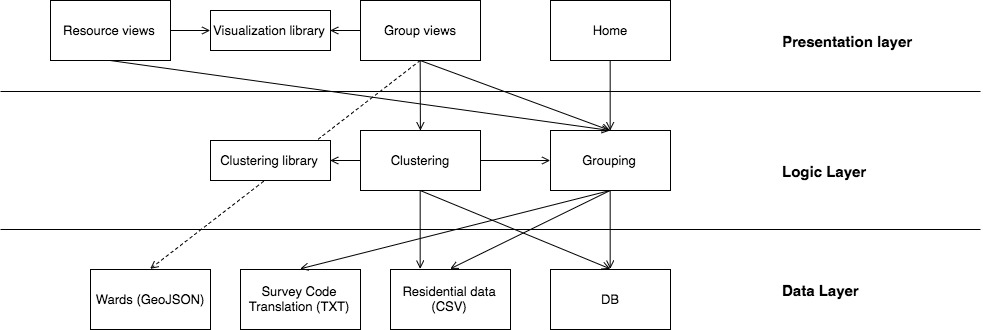
\includegraphics[scale=0.5]{FYP_Architecture}
\caption{System architecture diagram}
\end{figure}

The system will follow the three-layer architecture. \par
The data layer will consist of the following components:
\begin{itemize}
  \item \textbf{Ward}: a GeoJSON file containing the geographical boundaries of each ward
  \item \textbf{Survey Code Translation}: a text file formatted according to section \ref{preprocessing} containing the translations of the survey code to English text
  \item \textbf{Residential data}: a CSV file of the 2016 Lambeth Residential Survey
  \item \textbf{DB}: the database which includes Groups created by the user and groups\textsc{\char13} Clusters produced by the clustering algorithms (see  Appendix for more details)
\end{itemize}

The logic layer will consist of the following components:
\begin{itemize}
  \item \textbf{Clustering library}: a third-party library used by the Clustering component to cluster group data
  \item \textbf{Clustering}: performs clustering on a group and stores results in the database
  \item \textbf{Grouping}: creates groups and extracts groups from survey data
\end{itemize}

The presentation layer will consist of the following components (see section \ref{interface} for more details):
\begin{itemize}
  \item \textbf{Resource views}: shows visualizations data on each group for each question in the residential data set
  \item \textbf{Visualization library}: a third-party library used to create graph and map visualizations
  \item \textbf{Group views}: shows visualizations of groups and compares groups
  \item \textbf{Home}: main menu to choose which group to view
\end{itemize}

Though the original source of the Wards GeoJSON is from Lambeth\textquotesingle s open data website, it will be downloaded as a JSON file and stored as part of the source code of the application. Since the ward boundaries is unlikely to changing, storing the file in the source code is preferable as it will not depend on another server\textquotesingle s performance.\par

The Clustering component could be implemented separately and another clustering algorithm can be implemented without changing the Grouping component. 



\section{Algorithms}
Data analysis will be carried out by the system through data clustering. The clusters will be generated by the Clustering component and will be saved to the database. The default number of clusters is 1 and the user will be able to manipulate the number of clusters. \par

There are numerous clustering algorithms however, due to the categorical nature of the data, k-modes clustering will be used instead of the the usual k-means clustering. K-modes has been proven to be more effective in clustering categorical data (citation).

\section{User interface} \label{interface}
The system\textquotesingle s main goal is to present data and let the user interact with the user in an effective way. The following figures describe the interaction and design of the user interfaces.

\begin{figure}[h]
\centering
\includegraphics[scale=0.5]{FYP_InteractionDiagram.png}
\caption{Interaction diagram of the web application}
\end{figure}

The interaction diagram above describes the flow between the pages in the website. It is designed so that switching pages is done in the least number of clicks possible. This will be done through a navigation bar where most pages will be accessible. The group detail pages will only be accessible from the group\_detail.html page to avoid confusion with other groups\textsc{\char13} pages.\par

The following describes the functions of each page:
\begin{itemize}
  \item \textbf{index.html}: contains a list of links to all groups
  \item \textbf{group\_detail.html}: has visualizations of a group\textquotesingle s data through maps and charts (see section for more detail)
  \item \textbf{group\_compare.html}: compares all the groups to the average of the whole population of a data variable. This will visualize the comparison of the values of the cluster to the average value for that variable in the whole population (see section for more detail)
  \item \textbf{cluster\_compare.html}: compares the data on the clusters of a group, to the group and the whole population for each question (see section for more detail)
  \item \textbf{cluster\_stats.html}: lets the user change the number of clusters and shows differences, namely the means of an answer to a question, between each cluster (see section for more detail)
  \item \textbf{group\_new.html}: contains a form that adds a new group to the database
  \item \textbf{resources\_list.html}: lists links to residential survey questions
  \item \textbf{resources\_datafields.html}: shows visualizations of data on all groups for a survey question
\end{itemize}

*Note that variable is to denote the selected question and choice (i.e. Q11, Full-time employee) \par

This design gives the user different perspectives on a population. Namely, a group\textquotesingle s data (group\_detail.html), data of clusters within a group (cluster\_detail.html), differences between a group and its clusters (cluster\_compare.html, cluster\_stats.html) and differences between groups (resources\_datafields.html). These features are intended to enable the user to identify interesting trends within a specific group, groups or cluster which may not be possible with fewer interfaces. 

\section{Interface design} \label{sec:interfacedesign}
The pages in the interaction diagram are described in more detail in the following page designs. Since a large part of the system is about the presentation of data, the layout of the visualizations and interactions within pages, shown as annotations, were designed.

\begin{figure}[h]
\centering
\includegraphics[scale=0.3]{FYP_Screenshots1.png}
\caption{Page design for group\_detail.html and cluster\_compare.html}
\label{fig:FYP_Screenshots1}
\end{figure}

The page on figure \ref{fig:FYP_Screenshots1} is intended for the user to view the residential data which is visualized in graphs on the right-hand side of the page. Selecting a variable (i.e. a survey question and choice) on a graph will show its data on the map, on the left-hand side of the page, as a population density map. Each ward will be colored depending on the number of residents for which the resident chose the variable. This shows the user where residents who have chosen the variable live. Supporting the map is a bar chart of the number of residents for each ward who have chosen the variable which is ordered from greatest to least. This lets the user easily identify the distribution of the selected variable throughout the wards. The charts will follow functional requirements 3, which specifies which type of graph (e.g. bar chart, pie chart, etc.) to use for which type of question.\par

In addition, the meta-data about the data set used in the page is shown in the top left panel, which shows the number of residents in the group as a raw number and percentage and the source of the data.

\begin{figure}[h]
\centering
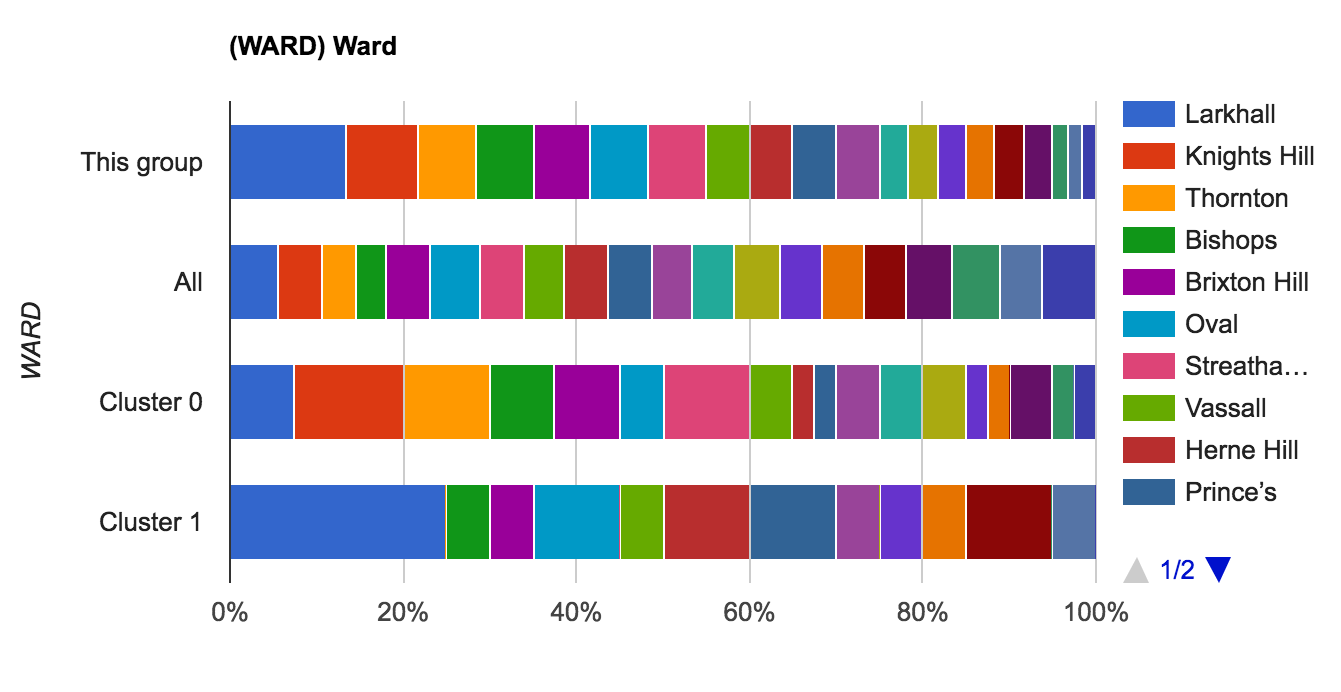
\includegraphics[scale=0.5]{comparison}
\caption{Chart for comparison of the data of the whole population, a group and its clusters}
\label{fig:comparison}
\end{figure}

The same page design is used for cluster\_compare.html except that the Question graphs will be in the form of stacked bar charts which show the question data on the whole population, the group and the clusters (see figure \ref{fig:comparison}). \par

The figure \ref{fig:comparison} is the visualization for the resources\_datafields.html page. However, the y-axis will instead be the groups in the database.

\begin{figure}[h]
\centering
\includegraphics[scale=0.3]{FYP_Screenshots2}
\caption{Page design for group\_compare.html}
\label{fig:FYP_Screenshots2}
\end{figure}

The page on figure \ref{fig:FYP_Screenshots2} will let the user compare the percent difference from the whole population using the following equation:\par

(Percent of the group\textquotesingle s population who answered selected question with selected choice-Percent of the overall population who answered selected question with selected choice)*100\par

Therefore groups more than 0\% has a bigger proportion of their population which have answered the selected variable and vice versa for groups less than 0\%. This may be an interesting visualization for some questions more than others.

\begin{figure}[h]
\centering
\includegraphics[scale=0.3]{FYP_Screenshots3}
\caption{Page design for cluster\_stats.html}
\label{fig:FYP_Screenshots3}
\end{figure}

The page on figure \ref{fig:FYP_Screenshots3} gives another perspective to the comparisons show in cluster\_compare.html. Instead of showing the all the data variables, the set of answers are consolidated into a mean. The user can compare means of a question for each cluster which will highlight the differences between each cluster which is not always obvious in cluster\_compare.html. The user may go back to cluster\_compare.html to the data in more detail.
